\documentclass{sig-alternate-05-2015}

\begin{document}

\title{Automated Test Case Generation}
\subtitle{Literature Review}

\numberofauthors{1}

\author{
\alignauthor
Patrick O'Connell \\
\email{proconne@ncsu.edu}
}

\maketitle

\begin{abstract}
This report reviews the motivation of automated test case generation and
discusses some of the challenges involved. It then outlines the main approaches
that have been attempted and describes some notable examples of each. Last, it
discusses possibilities for future research in the field.
\end{abstract}

\keywords{automated testing; search algorithms; genetic algorithms;
          constraint satisfaction}

\section{Introduction}

Testing is an important part of software development which can increase
confidence that software is free of defects and will work as intended. In
particular, unit tests are often able to isolate defects to a small part of the
codebase, which saves a lot of developer time compared to observing a bug as
the software is being used and having to determine which code is causing the
bug. Tests are also useful well after the relevant feature has been added, as
in addition to ensuring that the feature works properly initially, they can be
used to detect features which were broken with the addition of related code.

The main drawback to software testing is the time and effort taken to write the
test cases. It has been estimated that the typical project spends around half
of its time on testing \cite{beizer}. This is typically done manually by
someone with direct knowledge of the codebase, so the writing of test cases
requires a lot of programmer time which could alternatively be used on
something more productive.

Automated test case generation is the task of automatically generating
high-quality test cases, where ``high-quality'' is typically defined as having
high code coverage (roughly, the amount of the code explored through choosing
the right inputs to cover all branches) or some similar metric \cite{harman}.

This is, in general, a very challenging task. The space of all inputs to a
function is too large to simply iterate over and perform an exhaustive search,
especially when the input is of a structured type such as a list or tree. The
fact that branching instructions are discrete (control flow cannot partially
follow one path) makes maximizing code coverage a discrete optimization
problem, which are usually much more difficult than continuous ones.

In addition, the constraints describing whether control flow reaches a given
location are sometimes very specific (that is, they are satisfied for a small
fraction of the input space) and not readily apparent from a quick pass through
the source code. For example, a relatively simple constraint would be that in a
function which takes a list as an argument, a given line of code might be
reached only when the list is sorted except for the last element, and a
different parameter has a certain value. It would be very difficult for a
search algorithm to find a value that satisfies this constraint ``on
accident,'' and to extract this constraint from the code it is necessary to use
inefficient techniques such as symbolic execution.

\section{Search-Based Methods}

One possible approach to test case generation is to use a search algorithm
(usually local search) to find in the space of possible inputs the ones that
maximize code coverage \cite{anand}. The search operators depend on the type of
the inputs
to a function; they could be as simple as randomly changing one parameter when
they are integer-valued, but are more complicated for functions that, for
example, take as input a complex data structure.

Search methods are complicated by the fact that, because test case generation
is usually formulated as a discrete optimization problem, the objective
function does not improve smoothly as the search approaches an optimum.
Instead, the problem is characterized by sudden jumps when a constraint goes
from not being satisfied to being satisfied.

\subsection{Harmen Sthamer: \\The Automatic Generation of Software Test Data
            Using Genetic Algorithms}

One early attempt at using a search algorithm for test case generation was by
Harmen Sthamer in his PhD thesis \cite{sthamer}, which used a genetic algorithm
to find test
cases for several different types of simple example functions, and found that
the genetic algorithm outperformed a random search in terms of both runtime and
the number of test cases required for a certain amount of code coverage.

He had four stated hypotheses before he begun his work. The first was that a
genetic algorithm would outperform random search, which was the entire
motivation for the project. The second was that out of all of the parameters
for the genetic algorithm (population size, mutation rate, etc.) there would be
a setting for the parameters which would work well for a variety of functions
with different input types. This is highly desirable as the goal of automated
test case generation is to reduce manual effort, and requiring hand-tuning of
parameters for different functions would partially negate this. The third
hypothesis was that test generation would be successful for loops with varying
numbers of iterations: specifically no iterations, one, two and more than two.
The last hypothesis was that test cases generated would be adequate, as to be
confirmed by mutation analysis \cite{demillo1}. After some experimentation he
confirmed all of these hypotheses to be true.

The first type of function tested was functions with arithmetic and branch
instructions but no loops. Results on these functions were very good; random
testing did not do as well, mainly due to the noncontinuity and small size of
some subdomains (becuase of the arithmetic operations, sometimes a very precise
value had to be chosen for one input in order to reach a given branch).

Next, he tested on functions with loops that took complex data structures such
as lists as input. Several cases were identified where the genetic algorithm
was unable to find a satisfying test case due to complex constraints on the
input, but it again drastically outperformed random testing, achieving the same
code coverage with as few as one thirteenth of the tests.

Sthamer's evolutionary approach outperformed random testing, but was not
benchmarked against any more sophisticated methods.

\subsection{Gordon Fraser and Andrea Arcuri: \\Evolutionary Generation of Whole
            Test Suites}
\label{wts}

Most automated test case generation methods work by targeting a given part of
a codebase and running the generator many times, each run targeting a different 
part so that together the cases cover as much of the code as possible. Fraser
and Arcuri \cite{fraser-arcuri} develop an alternate method in which they
evolve the entire test suite at the same time.

This has many advantages over the traditional approach. If there is a part of
the code which is not reached for any input, a traditional search-based method
will typically be run until a maximum iteration count is reached, wasting a
significant amount of time. When evolving the entire test suite, however, no
time is spent directly on individual parts of the code, so none of the
generated suites will cover that part of the code but no time will be wasted in
order to determine that it could not be reached.

The same applies to code which is sometimes reached, but very rarely (and
therefore difficult to generate a test case for). If a reduction of the runtime
of the test generator is desired, the suite-based method can simply be run for
fewer iterations to find a set of easy to find test cases with as high coverage
as possible. With the traditional method, however, it is not known ahead of
time which cases will be hard to find.

In addition, when an input is chosen to cover one part of the code, it will
also naturally cover other parts. When generating individual test cases using
the traditional approach, this leads to wasted effort if a test case covering
the additional code has already been generated.

They benchmarked their approach on six large Java projects. Five were open
source projects, and to increase the variety of the test code they additionally
tested on an industrial case study project which Arcuri had previously
researched \cite{arcuri}. Using these six codebases, they compared the approach
to a modified
version of their own method that generated individual test
cases rather than test suites. They kept as many details as possible the same
between the two methods; they were interested in comparing case-based
generators to suite-based generators and not in comparing actual search
algorithms, so their goal in keeping the two methods similar was to isolate
the effect of changing the approach from case-based to suite-based. However,
this could impact the results, as it is not obvious that methods that would
work the best for suite-based generation would also work well for case-based
generation, so it is possible that the method they chose favored the
suite-based approach.

As both methods tested were randomized algorithms, the results can and will
vary between runs and it is necessary to ensure statistical significance of the
results. This was achieved using the Mann-Whitney U test with a significance
level of 0.05. They found that the test suite size required to achieve a
certain coverage was low averaged across all tests, with a statistically
significant improvement on most individual tests.

\begin{figure}
\center
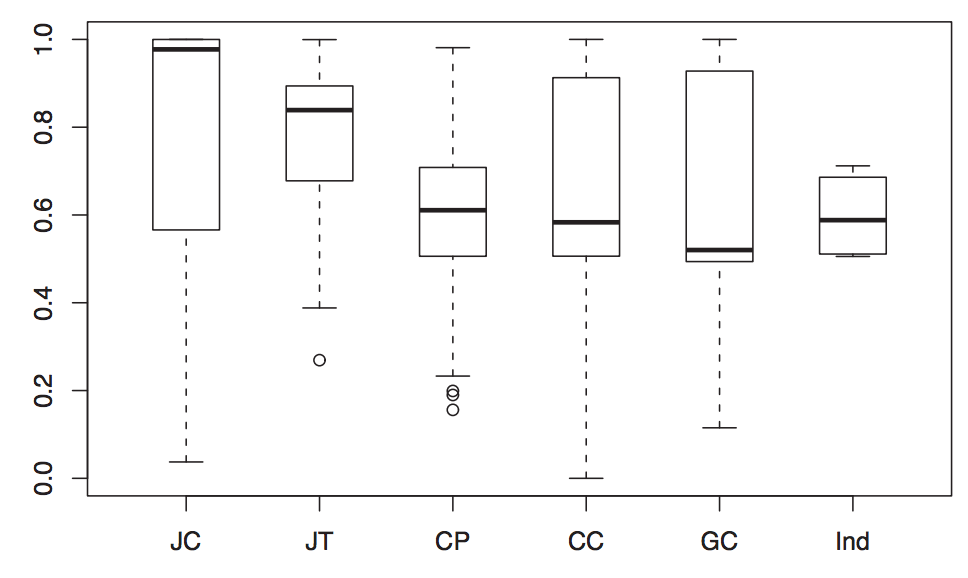
\includegraphics[scale=0.25]{plot.png}
\caption{Box plot of code coverage for each run on each test case}
\label{wts-plot}
\end{figure}

To visualize the results they calculated, for each test case and each run, the
statistical significance and plotted a box plot. An example is shown in Figure
\ref{wts-plot}, where a value of 1 means that their method had better coverage
and 0 means that the baseline was better. The middle quartiles of the box plot
can be viewed as a 50\% confidence interval.

\subsection{Nirmal Kumar Gupta and Mukesh Kumar Rohil: \\Improving GA Based
            Automated Test Data Generation Technique for Object Oriented
            Software}

Gupta and Rohil \cite{gupta} present a method which is also based on evolving
an entire test
suite using a genetic algorithm. Their contribution is that they explicitly
construct the control flow graph (CFG) of the program and assign weights to
each node which depend on how many times that node was reached across the test
suite. Mutations are then chosen with increased probability of reaching nodes
with low weights (nodes that were not visited as often) to increase code
coverage.

The authors claim that their method outperforms random testing, but do not give
any concrete results of random testing to compare their results to. In
addition, random testing is not a very ambitious benchmark to beat, as many
sophisticated methods which also beat random testing have been developed, and
it would be useful to compare their result to these. Despite the lack of
analysis, the method seems interesting and is probably worth looking into
further.

\subsection{Gordon Fraser and Andreas Zeller: \\Mutation-Driven Generation of
            Unit Tests and Oracles}
\label{ma}

Fraser and Zeller \cite{fraser-zeller} again use a genetic algorithm to
generate test cases, but use
a fitness evaluation function other than code coverage. They introduce
mutations (randomly created defects) in the code, and search for test cases
that give a different output from the original code and the mutated code. This
ensures that the chosen inputs are sensitive to small changes in the code,
which means that they will hopefully be able to detect other defects as well.

One motivation of mutation analysis is that it is closer to the actual goal of
software testing, and therefore hopefully more likely to generate test cases
that are actually useful. The goal of maximimum code coverage is somewhat
arbitrary, as the goal of reaching every point in the code is just a means to
an end; the actual focus of testing is to find defects, which is what mutation
analysis is designed to do.

The authors found that when compared to hand-written tests, their framework was
able to generate test cases that were both smaller and better at detecting
defects. Tests were performed on 10 open source Java libraries including
several Apache Commons projects, Google Collections and others. They displayed
their results using similar plots to those of Fraser and Arcuri, which show
the distribution over results for each test case. An example is shown in Figure
\ref{fz-plot}.

\begin{figure}
\center
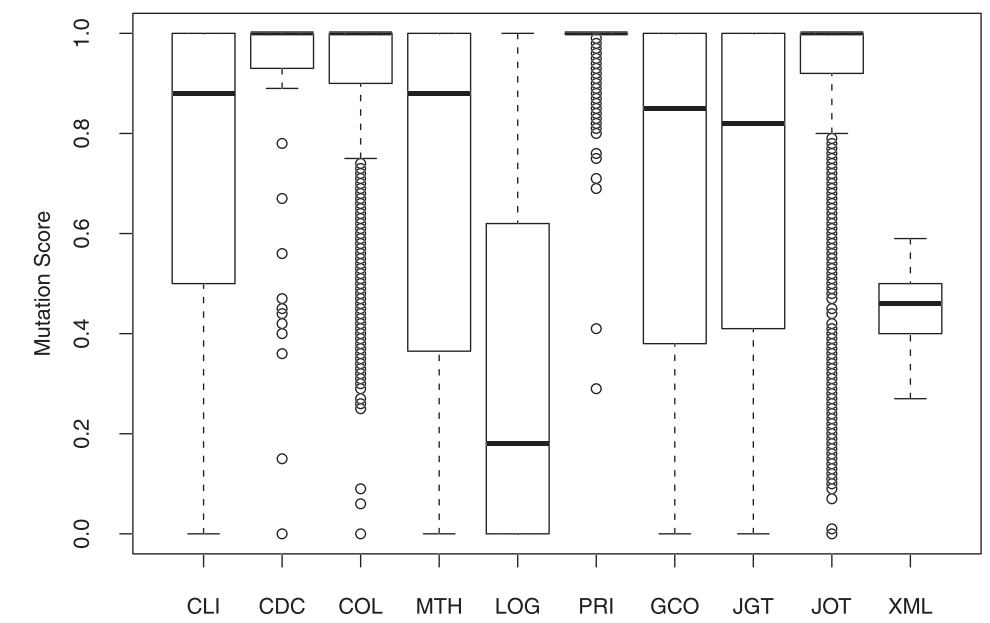
\includegraphics[scale=0.25]{fz-plot.png}
\caption{Box plot of mutation score for each run on each test case}
\label{fz-plot}
\end{figure}

\section{Other Methods}

\subsection{Matt Staats and Corina P\u{a}s\u{a}reanu: \\Parallel Symbolic
            Execution for Structural Test Generation}

One alternative method is parallel symbolic execution, in which a function run
is simulated without assigning concrete values to each variable. Instead,
variables are associated with symbolic values which, for each point in the
code, record which assignments to the variable lead to that code path. Test
cases can be generated by executing a function symbolicly and choosing a set
of inputs with sufficient combined coverage, which can be determined by
checking whether each input satisfies the conditions of various symbolic
values. Figure \ref{se-tree} shows the symbolic execution tree associated with
the code in Figure \ref{se-code}.

\begin{figure}
\center
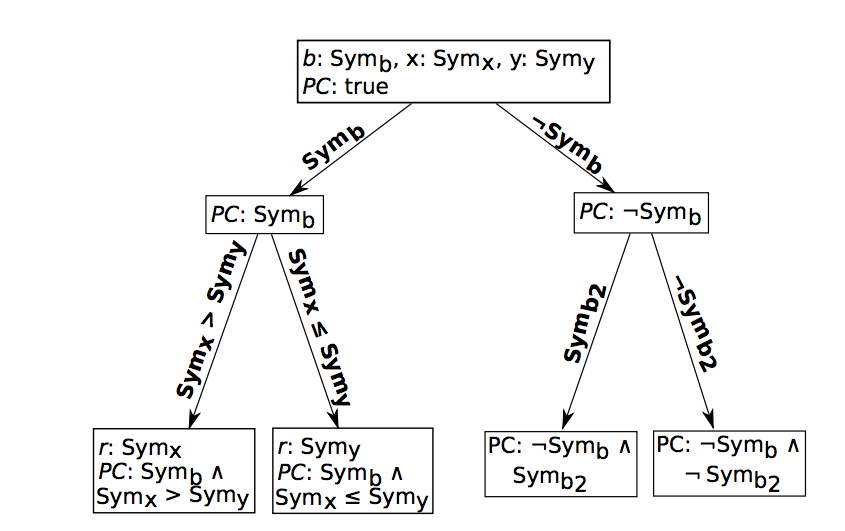
\includegraphics[scale=0.3]{se-tree.png}
\caption{Symbolic execution tree showing the constraints at each node}
\label{se-tree}
\end{figure}

\begin{figure}
\center
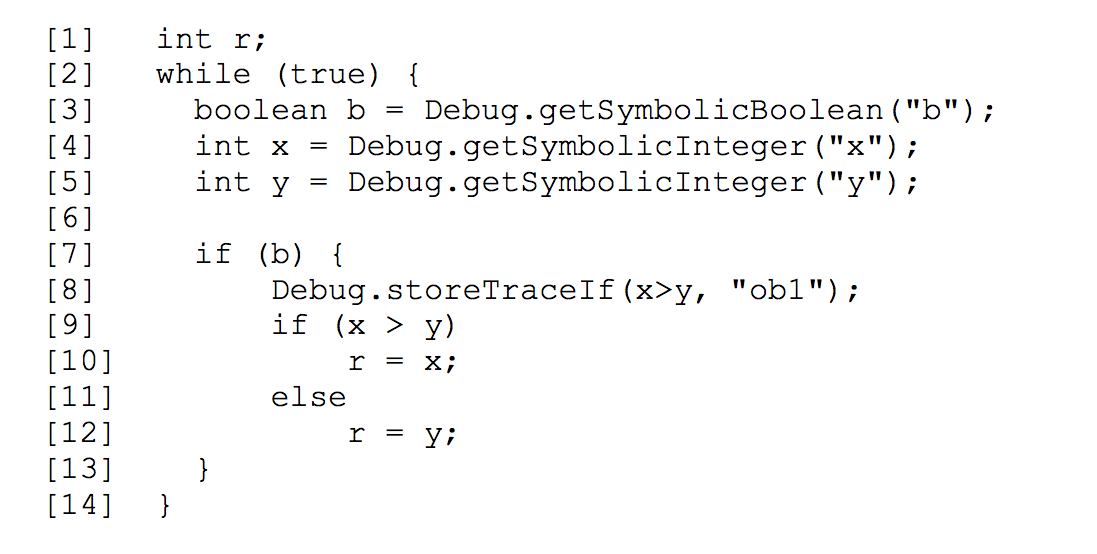
\includegraphics[scale=0.25]{se-code.png}
\caption{Code resulting in the symbolic execution tree in Figure \ref{se-tree}}
\label{se-code}
\end{figure}

This approach is very accurate and efficient for small, simple functions, but
does not scale well to larger and more complicated ones. The number of paths in
a function grow exponentially with its length assuming a constant density of
branching instructions, and complicated functions can lead to complicated
constraints which are intractable to satisfy.

Staats and P\u{a}s\u{a}reanu \cite{staats} use a method called ``selective
concretization'' to improve the running time of symbolic execution. Selective
concretization involves using some heuristics to concretize variables (convert
from a symbolic variable
to a concrete value) at dynamically chosen locations in the execution tree.
This reduces both the branching factor of the tree (and hence the number of
nodes) and the number of variables in the resulting constraint satisfaction
problems. Both of these asymptotically improve the runtime of symbolic
execution and allow it to handle larger problems.

They benchmark this method by comparing it to a random depth-first search of
the execution tree, and conclude that at the same depth and with the same
runtime, it obtains better code coverage. They used a parallel implementation
based on a custom client-server framework, and obtained a speedup that was
almost linear in the number of parallel threads.

\subsection{Richard DeMillo and A. Offutt: \\Constraint-Based Automatic Test
            Data Generation}

DeMillo and Offutt \cite{demillo} use mutation analysis as described in Section 
\ref{ma}, but
use a constraint satisfaction algorithm instead of an evolutionary one. They
use symbolic execution as described above with an extra condition associated
with each variable which represents whether the current state differs between
the original and mutated code.

One limitation is that due to the exponential runtime of constraint
satisfaction, this method is unable to be applied to large systems. The authors
mention decomposing the system into individual components and testing each
individually; however, this is sometimes impossible due to the system
architecture. In addition, the smaller the pieces into which the system must be
broken, the more redundant and overlapping test cases must be generated as
discussed in Section \ref{wts}.

Their method demonstrated promising results on the standard benchmark problem
\texttt{TRITYP} (triangle type) but this is a particularly small example, but
this took a non-negligible amount of time and (again due to the exponential
runtime of constraint satisfaction algorithms) it is likely that the largest
problems the approach is capable of solving are not much larger than
\texttt{TRITYP}.

\subsection{Jan Malburg and Gordon Fraser: \\Combining Search-Based and
            Constraint-Based Testing}

Malburg and Fraser \cite{malburg} combine search-based and constraint-based
methods by using
a genetic algorithm with a constraint solver during the mutation step which
ensures that mutation changes the input in a way that explores some other code
path. They report that this approach obtains many of the advantages of each
method with few of the disadvantages. The fact that these methods complement
each other and excel in areas where the other performs poorly was noted by
\cite{lakhotia}.

One of the main limitations of pure constraint-based test case generation is
the intractability of constraint satisfaction with a large number of
constraints, which means that these methods must be either very simplified or
applied to only a small segment of code, which is unable to take into account
global dependencies. The hybrid method of Malburg and Fraser, however, is able
to explore large regions of the input space (and therefore find a solution
which is hopefully closer to globally optimal) using the search algorithm while
only making local changes for which constraint satisfaction is tractable.

This addresses the problem with many other local search algorithms for test
case generation, which is that it is difficult to find improved solutions in
the local neighborhood due to discontinuities in the objective function.
Instead of addressing this through a more informative objective function, their
method modifies the mutation step to move in directions which are likely to
improve the solutions.

They compare their method to random testing, a simple genetic algorithm and a
constraint satisfaction approach, and obtain performance that is better than
all the others on most test cases, and tied for best on the others. Statistical
significance is ensured using the Mann-Whitney U test for the reasons given in
Section \ref{wts}.

\subsection{Arthur Baars et. al.: \\Symbolic Search-Based Testing}

Baars et. al. \cite{baars}, like Malburg and Fraser, use a hybrid method that
combines a search algorithm with symbolic techniques. They run partial symbolic
execution on the source code, which tracks some properties of the code path
previously taken but does not store the actual constraints representing that
path, which allows it to avoid the exponential blowup of number of paths
encountered when using full symbolic execution.

Given these metrics about the different code paths, they define a measure of
how close an input came to reaching a target part of the code, and use this
measure to define an alternative fitness function. This fitness function is
more informative as it indicates how close a test case came to meeting certain
coverage goals, as opposed to standard code coverage metrics which just take
into account whether a given line was executed or not.

The authors tested their fitness function using two different search
algorithms: a hill climbing algorithm named the Alternating Variable Method
\cite{korel} and an evolutionary approach by Wegener et. al. \cite{wegener}.

The authors use the Wilcoxon signed rank test to ensure statistical
significance. This differs from the Mann-Whitney U test used in other papers
in that instead of considering the results of each method to be an independent
sample, it uses matched pairs and directly compares the data points from each
method. This difference is justified because as opposed to the other papers
which are comparing multiple different methods, this paper compares a method to
itself with and without the modification of changing the fitness function, so
the pairs can be viewed as before and after data. Using this test they
determined that the modified fitness function improved code coverage for a
given test case size with a p-value of $2.2 \times 10^{-16}$, which means that
the results are extremely statistically significant.

One notable result was that the hill climbing method improved more from the
change than the genetic algorithm did. This is probably mainly due to the fact
that the hill climbing method had the lower performance initially, and
therefore the most room for improvement.

Because most other work on search-based test case generation has concerned the
search algorithm itself and for the most part has all used the same fitness
function (code coverage), this work is orthogonal to the approach of many other
methods. Therefore it does not directly address the limitations of other
methods, but rather gives a complementary technique which can be used in
conjunction with various search algorithms.

To conclude, the authors suggest that the fitness function they developed be
used in future research in search-based test case generation, as it
significantly outperformed traditional code coverage metrics.

\subsection{Casper S. Jensen, Mukul R. Prasad and Anders M\o ller: \\Automated
            Testing with Targeted Event Sequence Generation}

This paper \cite{jensen} addresses test case generation for mobile
applications, where rather
than scalar values or complex data structures, an input consists of a sequence
of UI events such as tapping an on-screen button. Their approach is based on
concolic execution, a hybrid of symbolic execution and concrete (or
``regular'') execution, similar to the approach of Staats and
P\u{a}s\u{a}reanu.

Next, given the output of concolic executive along with a target location in
the code, they locate the UI state corresponding to that code and perform a
backwards search in a state transition model of the UI in order to find a
sequence of actions that leads to that UI state, and consequently leads to that
code being executed. An example of a UI state transition model is shown in
Figure \ref{ui}.

\begin{figure}
\center
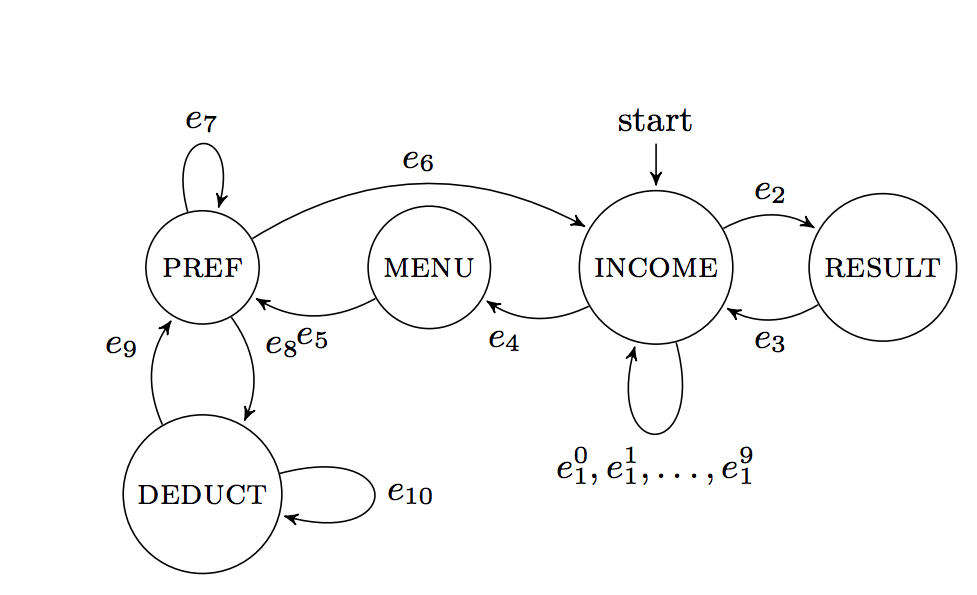
\includegraphics[scale=0.25]{ui.png}
\caption{State transition diagram of one of the applications tested by Jensen
         et. al.}
\label{ui}
\end{figure}

They concluded that this approach was successful, as it was able to find paths
to several hard to reach locations which were not found by random testing. An
advantage of their implementation was that it only required the bytecode of the
application that is being tested, and not the source code itself (black-box
testing).

This approach tests at the interface level in contrast with the previous
approaches, which unit tested individual parts of the code. Depending on the
type of application and the organization of the development team, this may be
either an advantage or a disadvantage.

\subsection{Rohan Sharma et. al.: \\A Comparison of Constraint-Based and
            \\Sequence-Based Generation of Complex Input Data Structures}

This paper \cite{sharma}, rather than directly address the task of test case
generation,
addresses the subproblem of generating complex data structures such as trees.
It does not attempt to maximize code coverage or any other test quality metric;
instead it simply compares methods for enumerating data structures of a given
type for use in test case generators.

The paper mentions test case generation as one of the primary motivations for
input structure generation, but the methods used have several limitations that
hinder their applicability to test generation. Primarily, they perform an
exhaustive enumeration of structures for a given size, which as previously
mentioned is typically much too large to search over. Possible future work to
move towards the goal of using this approach for automated testing would be to
define some fitness function and incorporate some sort of search algorithm to
find not all inputs, but the ones that maximize the objective function.

\section{Conclusions}

Based on the papers reviewed it seems to be the case that genetic algorithms
outperform constraint-based methods on all but the most trivial problems due to
the lack of scalability of constraint satisfaction algorithms. However, hybrid
methods seem to outperform both (or at least might have the potential to) and
represent a promising direction for future research. Malburg and Fraser claim
that their hybrid method achieves the advantages of both approaches with few of
the downsides, and the combining of multiple methods leads to a vast number of
possibilities, most of which have yet to be explored.

Another area which seems ideal for future work is the development of new
fitness functions. The lack of improvement in the immediate neighborhood of
most points due to the discrete nature of the code coverage objective causes
problems for local search algorithms, and Baars et. al. show promising results
using a modified fitness function based on a more meaningful metric of distance
from an optimum. There are still many possibilities for improved fitness
functions, which based on results so far should have a dramatic effect on
performance of search algorithms.

\bibliographystyle{abbrv}
\bibliography{paper}

\end{document}
